\documentclass[11pt,a4paper,twoside]{report}
\usepackage{amsmath,titlesec}
\usepackage{paralist}
\usepackage[scaled]{beramono}
\usepackage{colortbl}
\definecolor{gray-5}{gray}{0.95}
\definecolor{gray-10}{gray}{0.9}
\definecolor{gray-20}{gray}{0.8}
\definecolor{gray-30}{gray}{0.7}
\definecolor{gray-40}{gray}{0.6}
\definecolor{fadered}{rgb}{0.8824, 0.9529, 0.8745}
\usepackage{charter}
\usepackage{longtable}
\usepackage{multirow}
\usepackage[pdftex]{graphicx}
\usepackage{caption}
\usepackage[top=1in, bottom=1in, left=1in, right=1in]{geometry}
\usepackage[charter]{mathdesign}
\usepackage[utf8]{inputenc}
\usepackage[none]{hyphenat} 
\usepackage{float}
\usepackage[final]{pdfpages}
% \usepackage{setspace}
\usepackage[charter]{mathdesign}
% \usepackage[small]{caption}
% \usepackage{abstract}
% \usepackage{lineno}

\usepackage{listings} 
\lstset{numbers=left, numberstyle=\scriptsize\ttfamily, numbersep=10pt, captionpos=b} 
\lstset{backgroundcolor=\color{gray-5}}
\lstset{basicstyle=\small\ttfamily}
\lstset{framesep=4pt}
\lstset{language={}}
\newcommand{\inlineCode}{\lstinline[basicstyle=\normalsize\ttfamily]}
\newcommand{\first}[1]{{\vspace{1ex}}{\Large \textbf{#1}}{\vspace{1ex}}}
\newcommand{\second}[1]{{\vspace{1ex}}{\large \textbf{#1}}}
\newcommand{\tabspace}[0]{\vspace{2mm}}
\newcommand{\cvsubheader}[1]{\multicolumn{2}{@{}l}{\second{#1}} \\ \nopagebreak[4]}
\newcommand{\cvitem}[1]{\input{../../common/#1}}
\newcommand{\cvtitle}[2]{#1 & \textbf{#2} \\ \nopagebreak}
\renewcommand\bibname{References}

\usepackage[colorlinks=true,linkcolor=black,citecolor=black,urlcolor=black,filecolor=black,bookmarks=true]{hyperref}
\hypersetup{
pdfauthor = {Michael Specht},
pdftitle = {},
pdfsubject = {},
pdfkeywords = {},
pdfcreator = {LaTeX},
pdfproducer = {pdflatex}}


    \makeatletter 
    \def\cleardoublepage{\clearpage\if@twoside \ifodd\c@page\else% 
    \hbox{}% 
    \thispagestyle{empty}
    \newpage% 
    \if@twocolumn\hbox{}\newpage\fi\fi\fi} 
    \makeatother

% Definition from latex.ltx modified
% \makeatletter
% \renewcommand*{\cleardoublepage}{%
%   \clearpage
%   \if@twoside
%     \ifodd\c@page
%       \hbox{}%
%       \newpage
%       \if@twocolumn
%         \hbox{}%
%         \newpage
%       \fi
%     \fi
%   \fi
% }
% \makeatother

\fboxsep0pt
\fboxrule0.05pt

\newcommand{\image}[5]{
  \begin{figure}[htbp]
    \centering
    \includegraphics[width=#3\textwidth]{#2}
    \caption[#5]{#4}
    \label{fig:#1}
  \end{figure}
}

\newcommand{\imageFrame}[5]{
  \begin{figure}[htbp]
    \centering
    \fbox{
      \includegraphics[width=#3\textwidth]{#2}
    }
    \caption[#5]{#4}
    \label{fig:#1}
  \end{figure}
}


\usepackage{setspace}
\usepackage{fancyhdr}
\usepackage{wrapfig}
% \renewcommand{\chaptermark}[1]{\markleft{#1}{}}
% \renewcommand{\sectionmark}[1]{\markright{#1}{}}
% \fancyhead[C]{\rightmark}
% \renewcommand{\headrulewidth}{0pt}
% \renewcommand{\footrulewidth}{0pt}
\def \cre{{\em C.~reinhardtii}}
\def \dmel{{\em D.~melanogaster}}
\def \chlre{{\em Chlamydomonas reinhardtii}}

\def \fmfour{FM4}
\def \augno{AUGUSTUS}
\def \augyes{AUGUSTUS/GPF}
\def \etal{{\em et al.}}
\def \denovo{{\em de novo}}
\def \insilico{{\em in silico}}
\def \mz{{\em m/z}}

\hyphenation{AUGUSTUS}
\setlength{\parskip}{2mm}
\setlength{\parindent}{0mm}
\renewcommand{\baselinestretch}{1.4} 
\renewcommand{\arraystretch}{1.4} 

\renewcommand{\headrulewidth}{0.25pt}

\pagestyle{fancy}

\renewcommand{\chaptermark}[1]{\markboth{#1}{}}
\renewcommand{\sectionmark}[1]{\markright{#1}}

%\setlength{\marginparwidth}{1.5cm}
%\newcommand{\note}[1]{\marginpar{\color{gray-40}\footnotesize \flushleft #1}}
\newcommand{\note}[1]{}

\newcommand{\imageCourtesy}[2]{Image courtesy of #1 \cite{#2}.}

\fancyhf{}
\fancyhead[EL,OR]{\thepage}
\fancyhead[ER]{\leftmark}
\fancyhead[OL]{\rightmark}
\fancypagestyle{plain} {
  \fancyhf{}
  \renewcommand{\headrulewidth}{0pt}
}

\lstnewenvironment{todo}{\lstset{numbers=none,frame=none,backgroundcolor=\color{fadered}}}{}
\pagestyle{empty}

% Code for creating empty pages
% No headers on empty pages before new chapter
% \makeatletter
% \def\cleardoublepage{\clearpage\if@twoside \ifodd\c@page\else
%     \hbox{}
%     \thispagestyle{plain}
%     \newpage
%     \if@twocolumn\hbox{}\newpage\fi\fi\fi}
% \makeatother \clearpage{\pagestyle{plain}\cleardoublepage}


\begin{document}
% \pagewiselinenumbers

\includepdfset{pages=-,noautoscale}

\begin{center}

\includegraphics[width=0.5\textwidth]{figures/wwu-logo-black.jpg}

{\Large Institut f\"ur Biologie und Biotechnologie der Pflanzen}

\vspace*{5cm}

% {\bf \Huge {\em Chlamydomonas reinhardtii} from the computational proteomics perspective}
{\bf \Huge Novel high-throughput data analysis strategies in computational proteomics and proteogenomics}

\vspace*{4cm}

{\Large Inaugural-Dissertation zur Erlangung des Doktorgrades der
Naturwissenschaften im Fachbereich Biologie der
Mathematisch-Naturwissenschaftlichen Fakult\"at der
\mbox{Westf\"alischen Wilhelms-Universit\"at M\"unster}}

\vspace*{2cm}

{\Large vorgelegt von}

{\LARGE \bf Michael Specht}

{\Large aus Magdeburg}

{\LARGE April 2011}

\end{center}

\cleardoublepage

\vspace*{550pt}

Dekan: Prof. Dr. Christian Kl\"ambt \newline
Erster Gutachter: Prof. Dr. Michael Hippler \newline
Zweite Gutachterin: Prof. Dr. Simone K\"onig \newline
Tag der m\"undlichen Pr\"ufung: \newline
Tag der Promotion: \newline

\cleardoublepage

\vspace*{200pt}
\begin{flushright}
{\Large\em
To my family, the great life amplifier: \\
Jule, Charlotte \& Leo
}
\end{flushright}

% \clearpage

% \begin{abstract}
% This is the abstract. Lots of hacking and MS here.
% \end{abstract}

% {\bf Abbreviations and acronyms used in the report:}
% 
% DSCAM -- down syndrome cell adhesion molecule, 
% FDR -- false discovery rate, 
% GPF -- Genomic Peptide Finder, 
% MS -- mass spectrometry,
% MS/MS -- tandem mass spectrometry,
% PSM -- peptide/spectral match

\fancypagestyle{plain}{
\fancyhf{}
\renewcommand{\headrulewidth}{0.25pt}
% \renewcommand{\footrulewidth}{0.5pt}
\fancyfoot[EL,OR]{\thepage}
\fancyhead[EL]{\leftmark}
\fancyhead[OR]{\rightmark}
}

\cleardoublepage
\setcounter{tocdepth}{2}
\setcounter{secnumdepth}{2}
\tableofcontents

\clearpage

% ==============================================================
\chapter{Introduction}
% ==============================================================

The proteome is defined as the set of proteins present in a cell, tissue, or
organism at a defined time point and under certain conditions.

\begin{figure}[h]
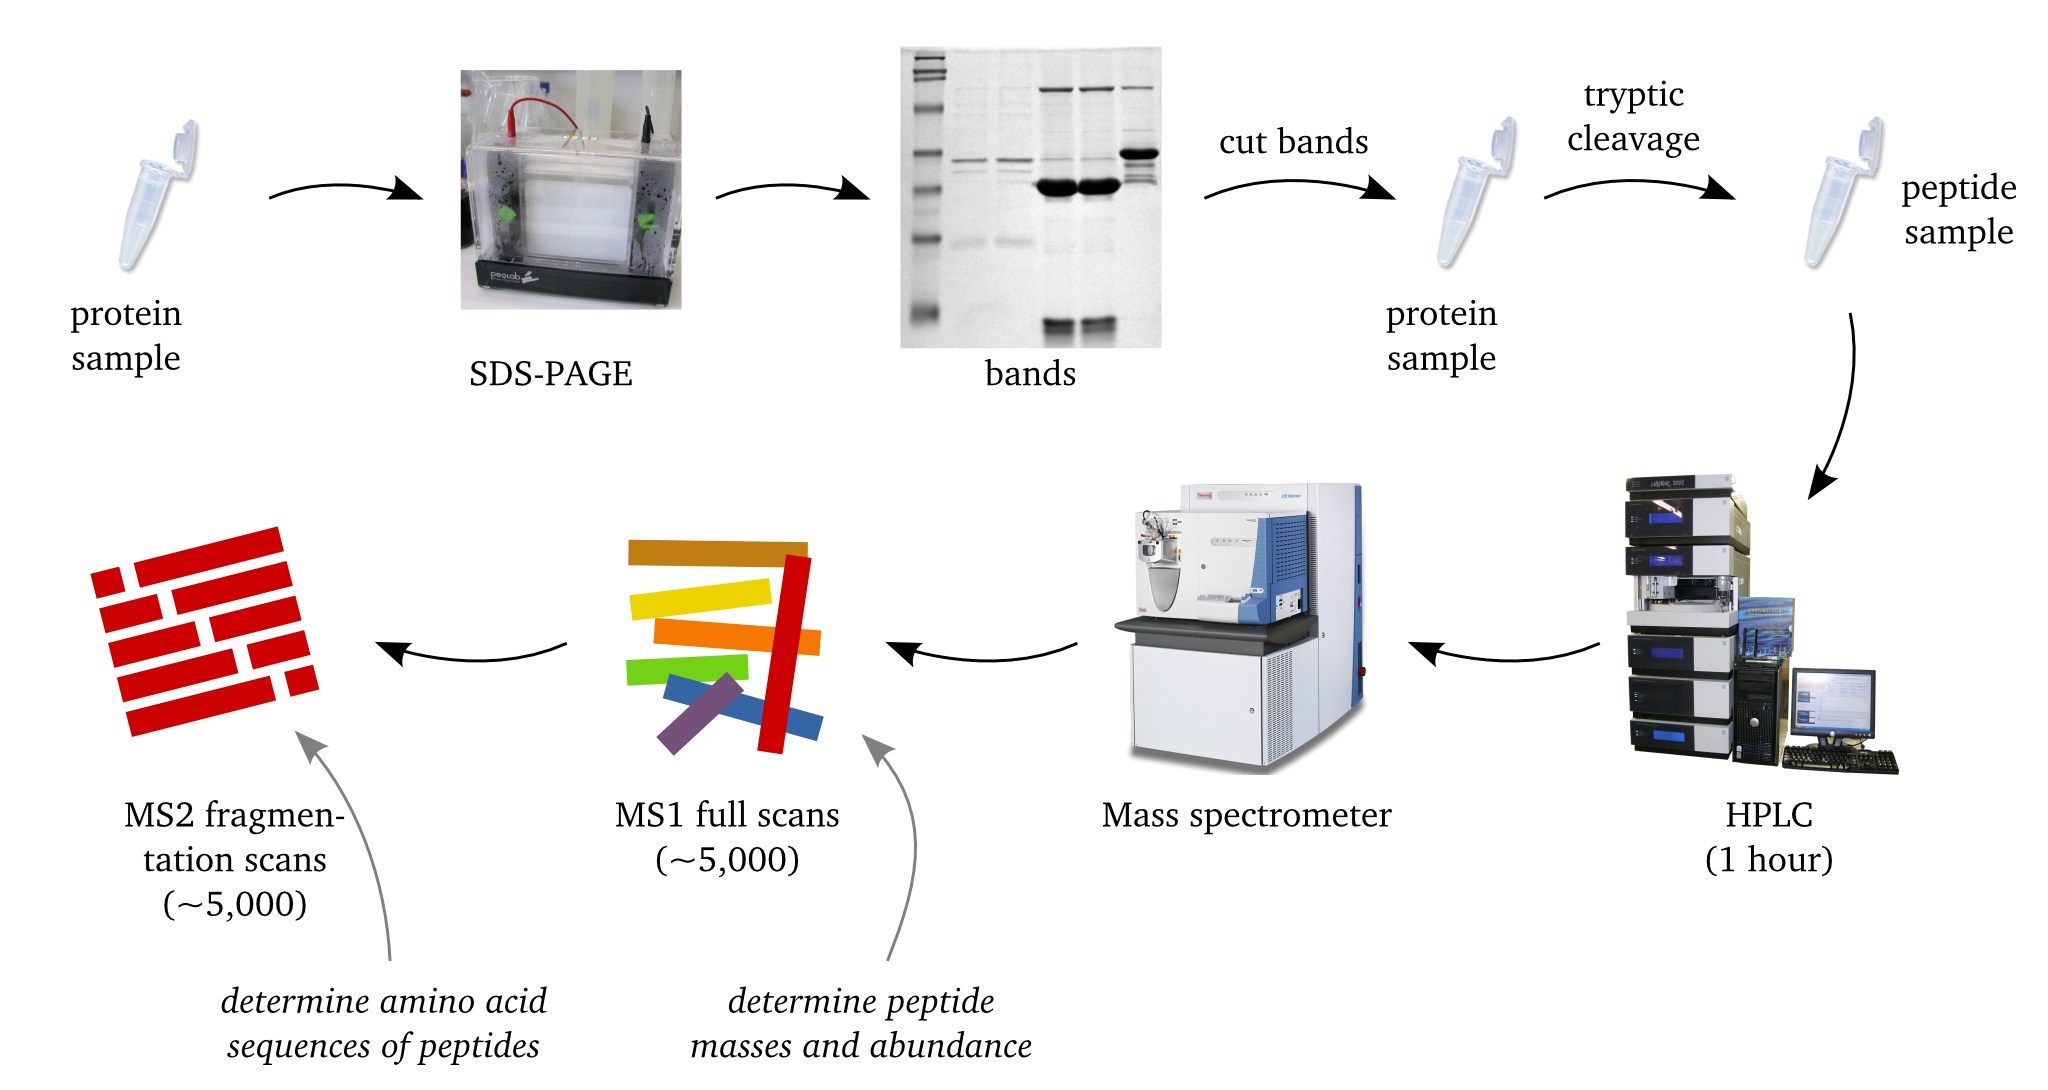
\includegraphics[width=\textwidth]{figures/Proteomics.jpg}
\caption{
{\bf Caption.} 
Caption here.
}
\label{fig:proteomics-overview}
\end{figure}

% --------------------------------------------------------------
\section{Acquisition of mass spectrometric data}
% --------------------------------------------------------------

\subsection{Preprocessing of biological samples}

\subsection{Ionization of molecules}

\subsection{Mass analysis}

\subsection{Mass spectra}

\subsubsection{Full scans (MS)}

\begin{figure}[h]
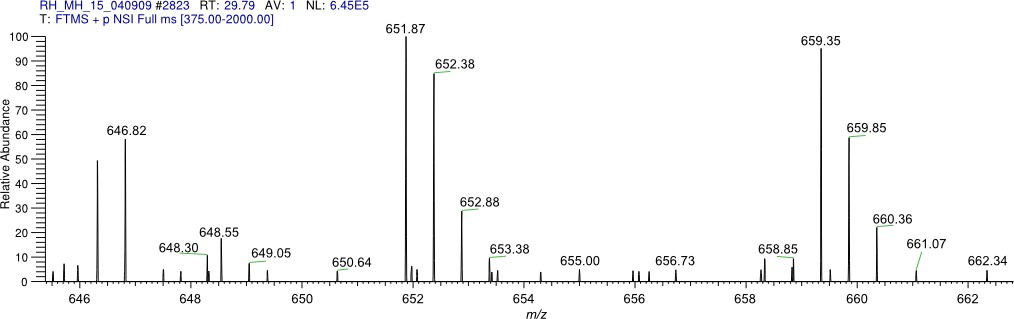
\includegraphics[width=\textwidth]{figures/ms1-scan.jpg}
\caption{
{\bf Example of a full scan.} 
Caption here.
}
\label{fig:full-scan}
\end{figure}

\subsubsection{Fragmentation scans (MS/MS)}

\begin{figure}[h]
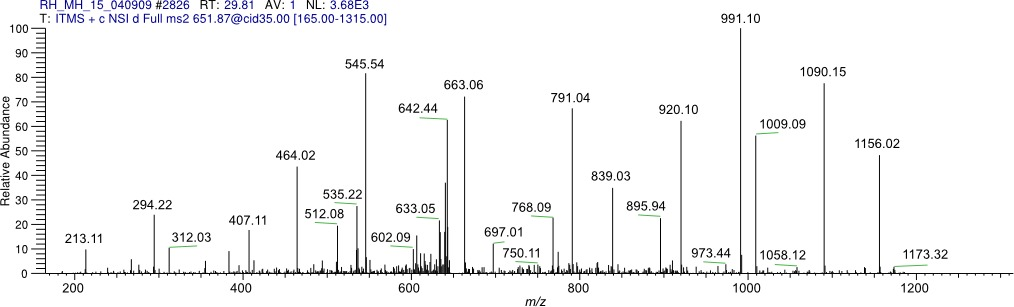
\includegraphics[width=\textwidth]{figures/ms2-scan.jpg}
\caption{
{\bf Example of a fragmentation scan.} 
Caption here.
}
\label{fig:fragmentation-scan}
\end{figure}

\begin{figure}[h]
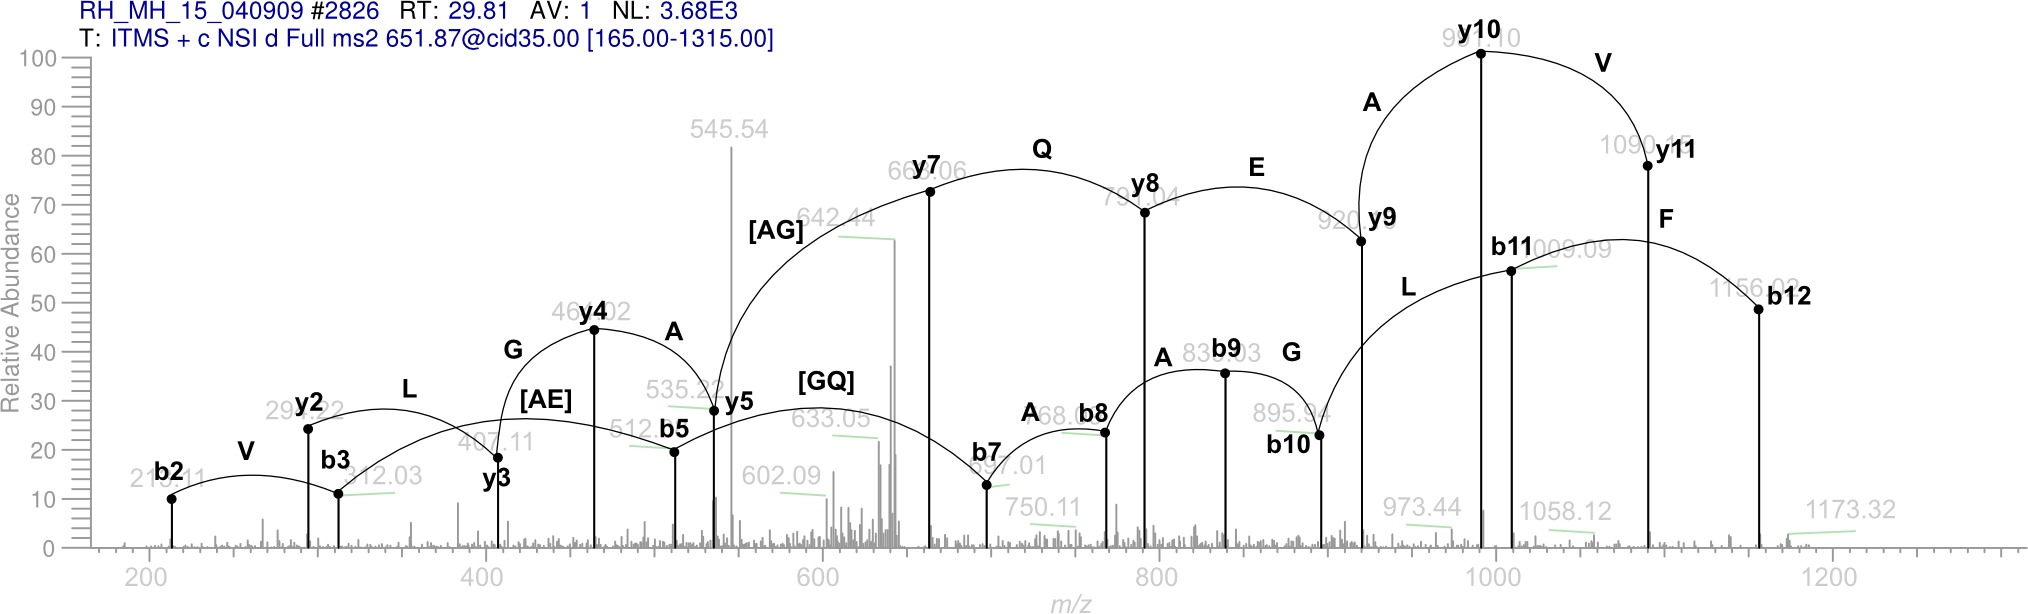
\includegraphics[width=\textwidth]{figures/ms2-scan-b-y-1.jpg}
\caption{
{\bf Fragmentation scan with b and y ion series mass ladders superimposed.} 
Caption here.
}
\label{fig:fragmentation-scan-b-y}
\end{figure}


% --------------------------------------------------------------
\section{Data evaluation}
% --------------------------------------------------------------

\subsection{Databases}

\subsubsection{Genome sequences}

\subsubsection{Protein databases}

\subsection{Identification}

\subsubsection{Peptide mass fingerprinting}

\subsubsection{Database search}

\subsubsection{De novo sequencing}

\subsection{Quantitation}

\subsubsection{Chemical labeling}
 
\subsubsection{Metabolic labeling}

\subsubsection{Label-free quantitation}

% --------------------------------------------------------------
\section{Proteogenomics}
% --------------------------------------------------------------

% --------------------------------------------------------------
\section{Chlamydomonas reinhardtii}
% --------------------------------------------------------------

\subsection{Anaerobic metabolism}

% --------------------------------------------------------------
\section{Thalassiosira oceanica}
% --------------------------------------------------------------

\subsection{Iron deficiency}

% ==============================================================
\chapter{Specific aims}
% ==============================================================

% ==============================================================
\chapter{Publications}
% ==============================================================

The following publications are presented in this thesis:

\begin{enumerate}
\item 
{\bf Proteomics to go: Proteomatic enables the user-friendly creation of versatile MS/MS data evaluation workflows.}

Michael Specht, Sebastian Kuhlgert, Christian Fufezan and Michael Hippler

Bioinformatics 2011; doi: 10.1093/bioinformatics/btr081 (in press).

\item
{\bf Characterizing the anaerobic response of Chlamydomonas reinhardtii by quantitative proteomics.}

Mia Terashima, Michael Specht, Bianca Naumann-Busch and Michael Hippler

Mol Cell Proteomics, 9(7), 2010: 1514-32.

\item
{\bf The chloroplast proteome: A concise survey form the {\em Chlamydomonas reinhardtii} perspective}

Mia Terashima, Michael Specht and Michael Hippler

2011, in minor revision.

\item
{\bf Concerted action of the new Genomic Peptide Finder and AUGUSTUS allows for automated proteogenomic annotation of the {\em Chlamydomonas reinhardtii} genome.}

Michael Specht, Mario Stanke, Mia Terashima, Bianca Naumann-Busch, Ingrid Jan\"sen, Ricarda H\"ohner, Erik F.~Y.~Hom, Chun Liang and Michael Hippler

Proteomics (2011), in press.

\item
{\bf T. oceanica paper with Markus Lommer}

\item
{\bf p3d -- Python module for structural bioinformatics}

Christian Fufezan and Michael Specht

BMC Bioinformatics (2009) 10:258.

\end{enumerate}

% --------------------------------------------------------------
\cleardoublepage
\section{Proteomics to go: Proteomatic enables the user-friendly creation of versatile MS/MS data evaluation workflows}
% \markboth{Proteomics to go: Proteomatic enables the user-friendly creation of versatile MS/MS data evaluation workflows}{Proteomics to go: Proteomatic enables the user-friendly creation of versatile MS/MS data evaluation workflows}
% \addcontentsline{toc}{section}{Proteomics to go: Proteomatic enables the user-friendly creation of versatile MS/MS data evaluation workflows}

Michael Specht, Sebastian Kuhlgert, Christian Fufezan and Michael Hippler

Bioinformatics 2011; doi: 10.1093/bioinformatics/btr081 (in press).

\subsection*{Contributions}

\begin{itemize}
\item design and implementation of Proteomatic
\item main contribution to the text
\item creation of figures
\item corresponding authorship
\end{itemize}

% \cleardoublepage
% 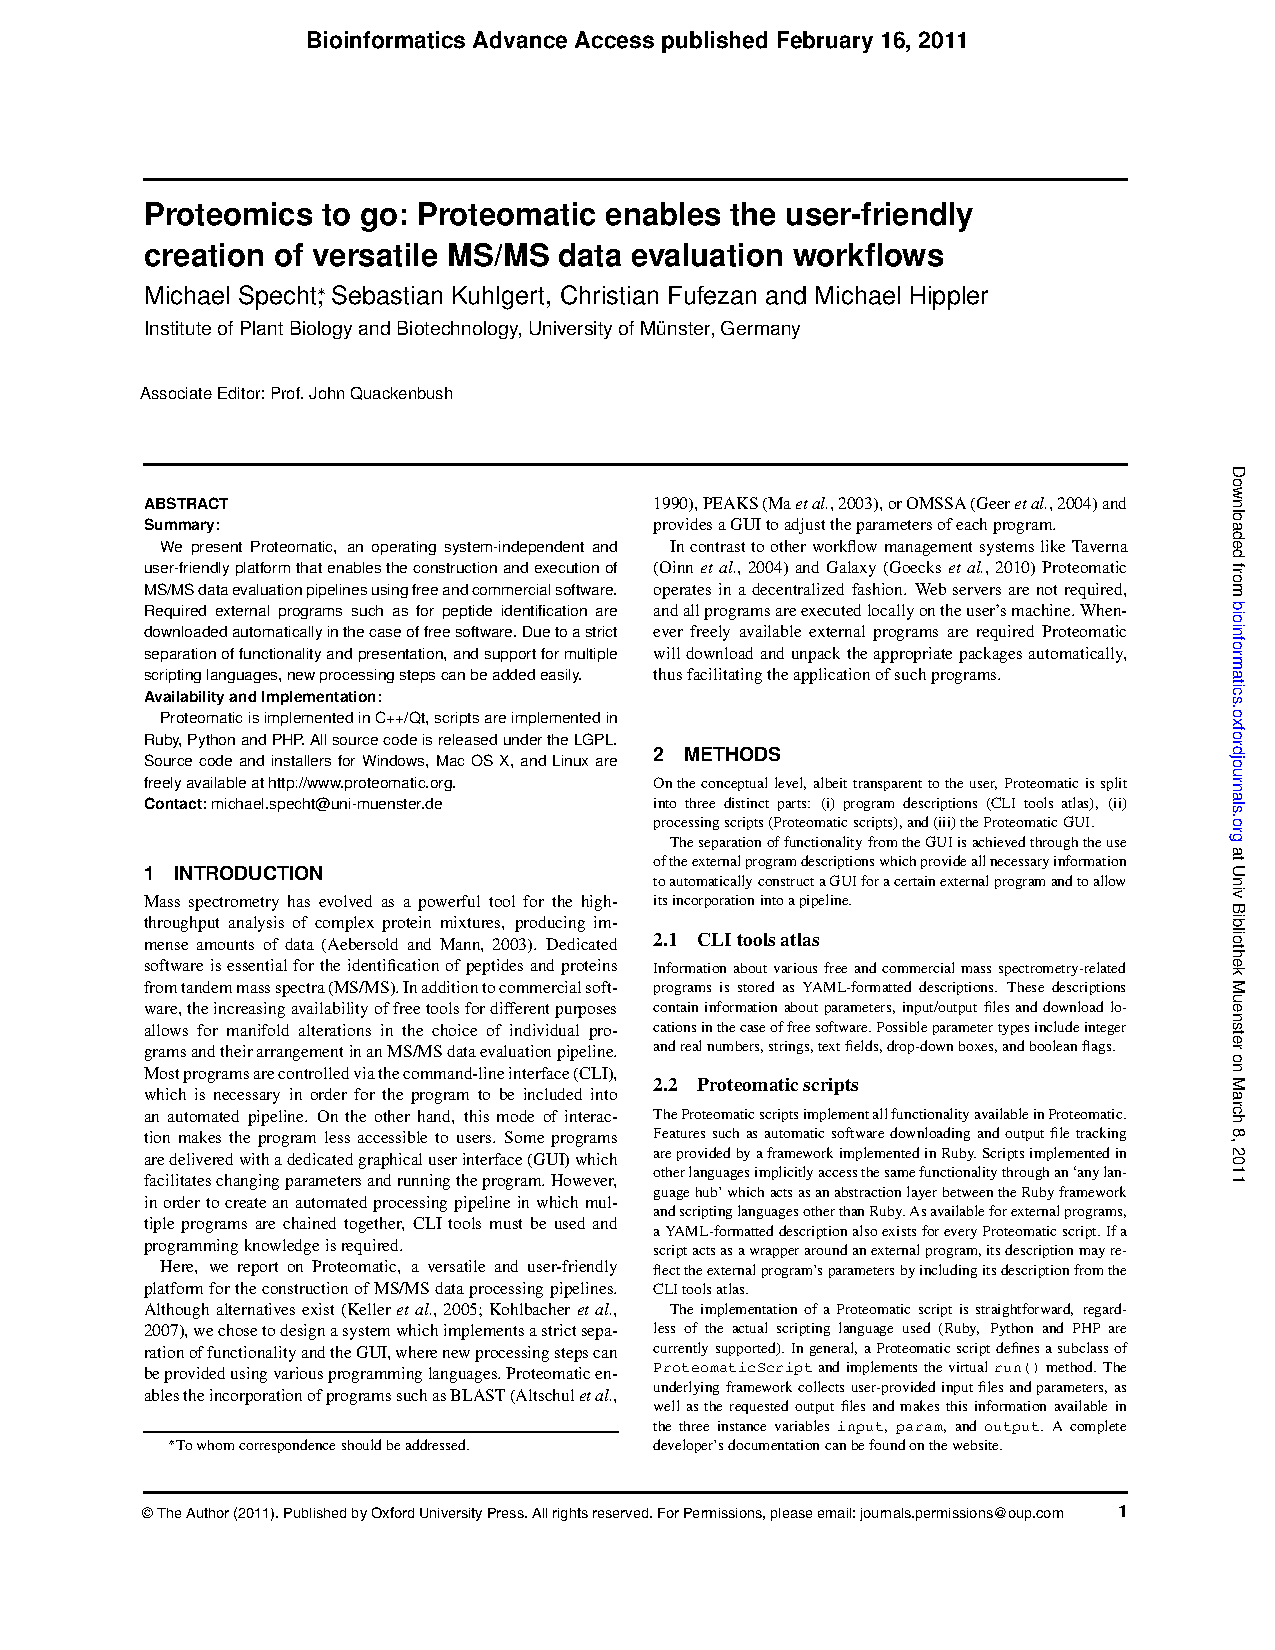
\includepdf{publications/proteomatic-2011.pdf}

% --------------------------------------------------------------
\cleardoublepage
\section{Characterizing the anaerobic response of {\em Chlamydomonas reinhardtii} by quantitative proteomics}
% \markboth{Characterizing the anaerobic response of {\em Chlamydomonas reinhardtii} by quantitative proteomics}{Characterizing the anaerobic response of {\em Chlamydomonas reinhardtii} by quantitative proteomics}
% \addcontentsline{toc}{section}{Characterizing the anaerobic response of {\em Chlamydomonas reinhardtii} by quantitative proteomics}
% --------------------------------------------------------------

\subsection*{Contributions}

\begin{itemize}
\item what was it, then?
\end{itemize}

% \cleardoublepage
% 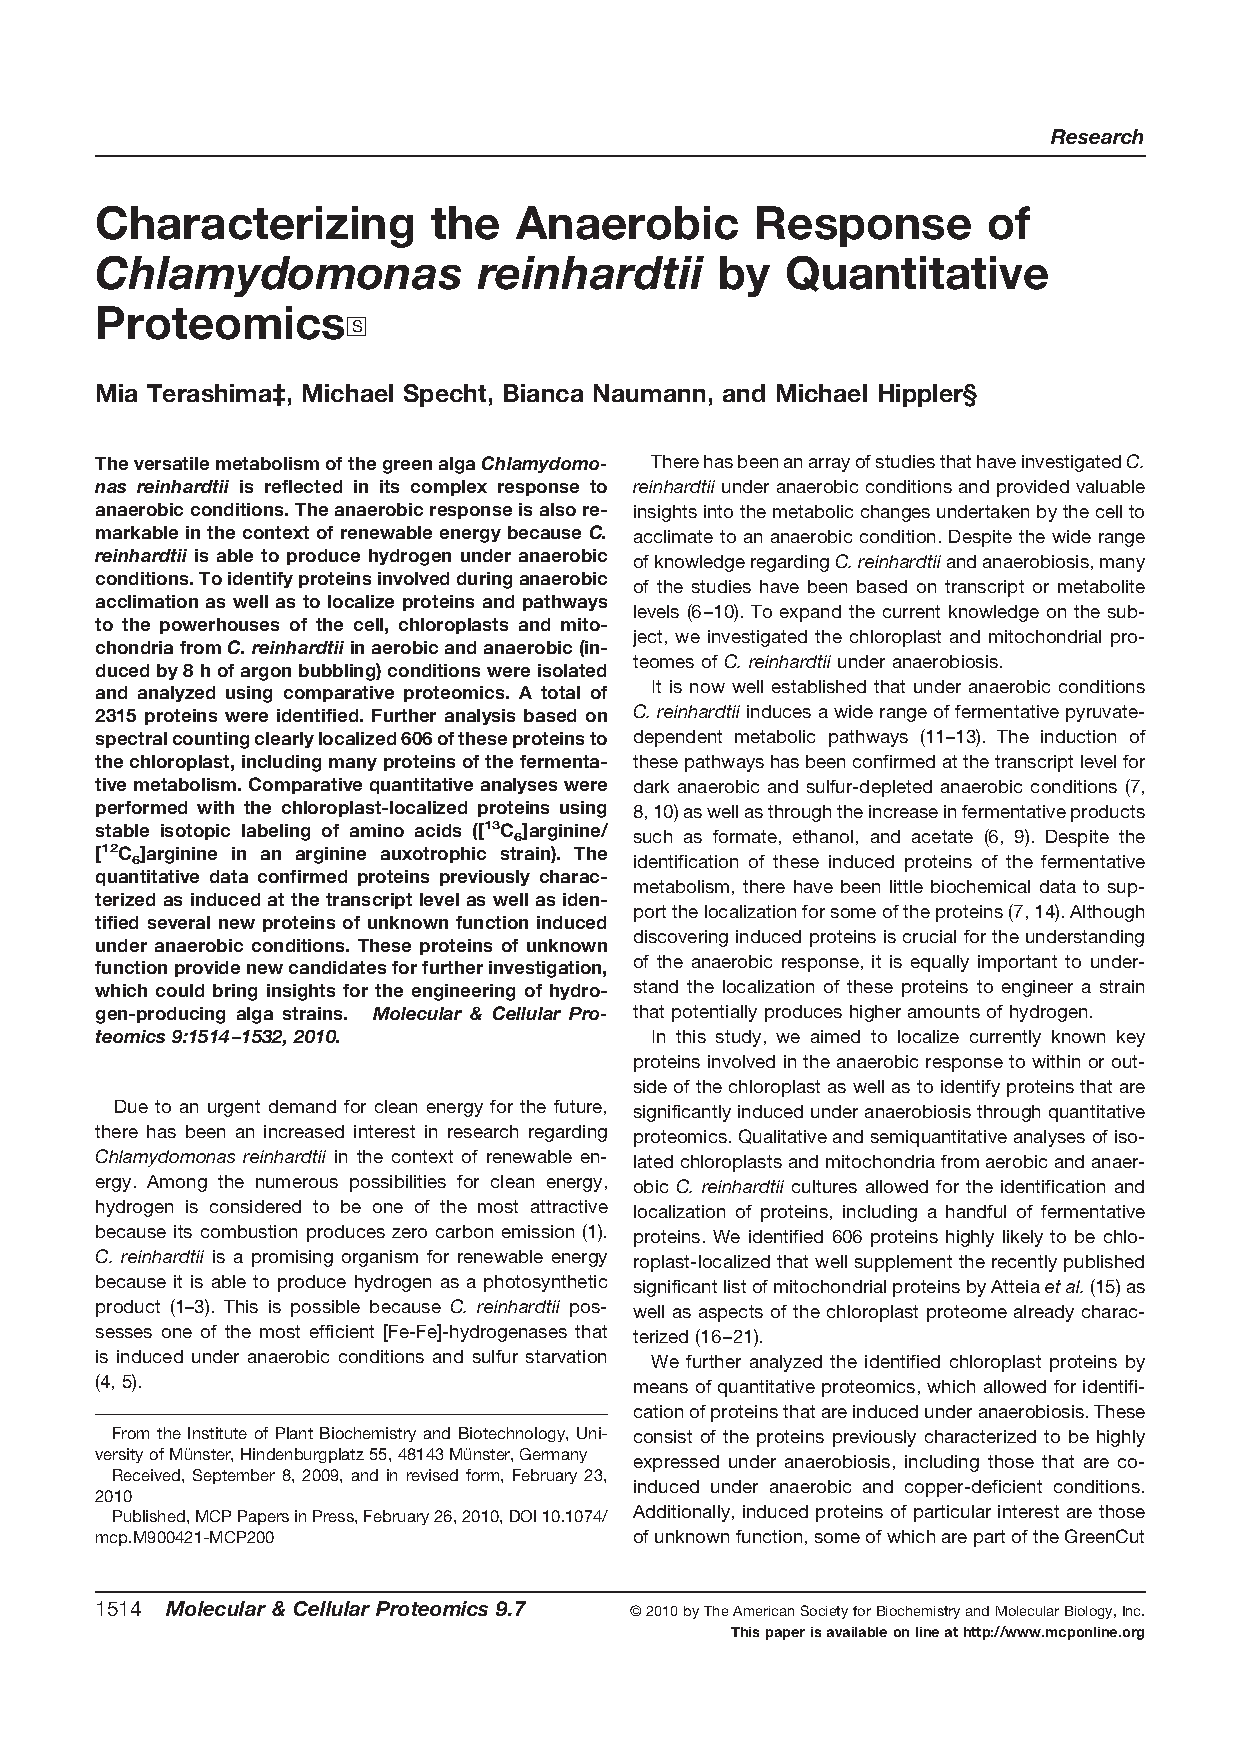
\includepdf{publications/terashima-2010.pdf}

% --------------------------------------------------------------
\cleardoublepage
\section{The chloroplast proteome: A concise survey form the {\em Chlamydomonas reinhardtii} perspective}
% \markboth{The chloroplast proteome: A concise survey form the {\em Chlamydomonas reinhardtii} perspective}{The chloroplast proteome: A concise survey form the {\em Chlamydomonas reinhardtii} perspective}
% \addcontentsline{toc}{section}{The chloroplast proteome: A concise survey form the {\em Chlamydomonas reinhardtii} perspective}
% --------------------------------------------------------------

\subsection*{Contributions}

\begin{itemize}
\item what was it, then?
\end{itemize}

% \cleardoublepage
% 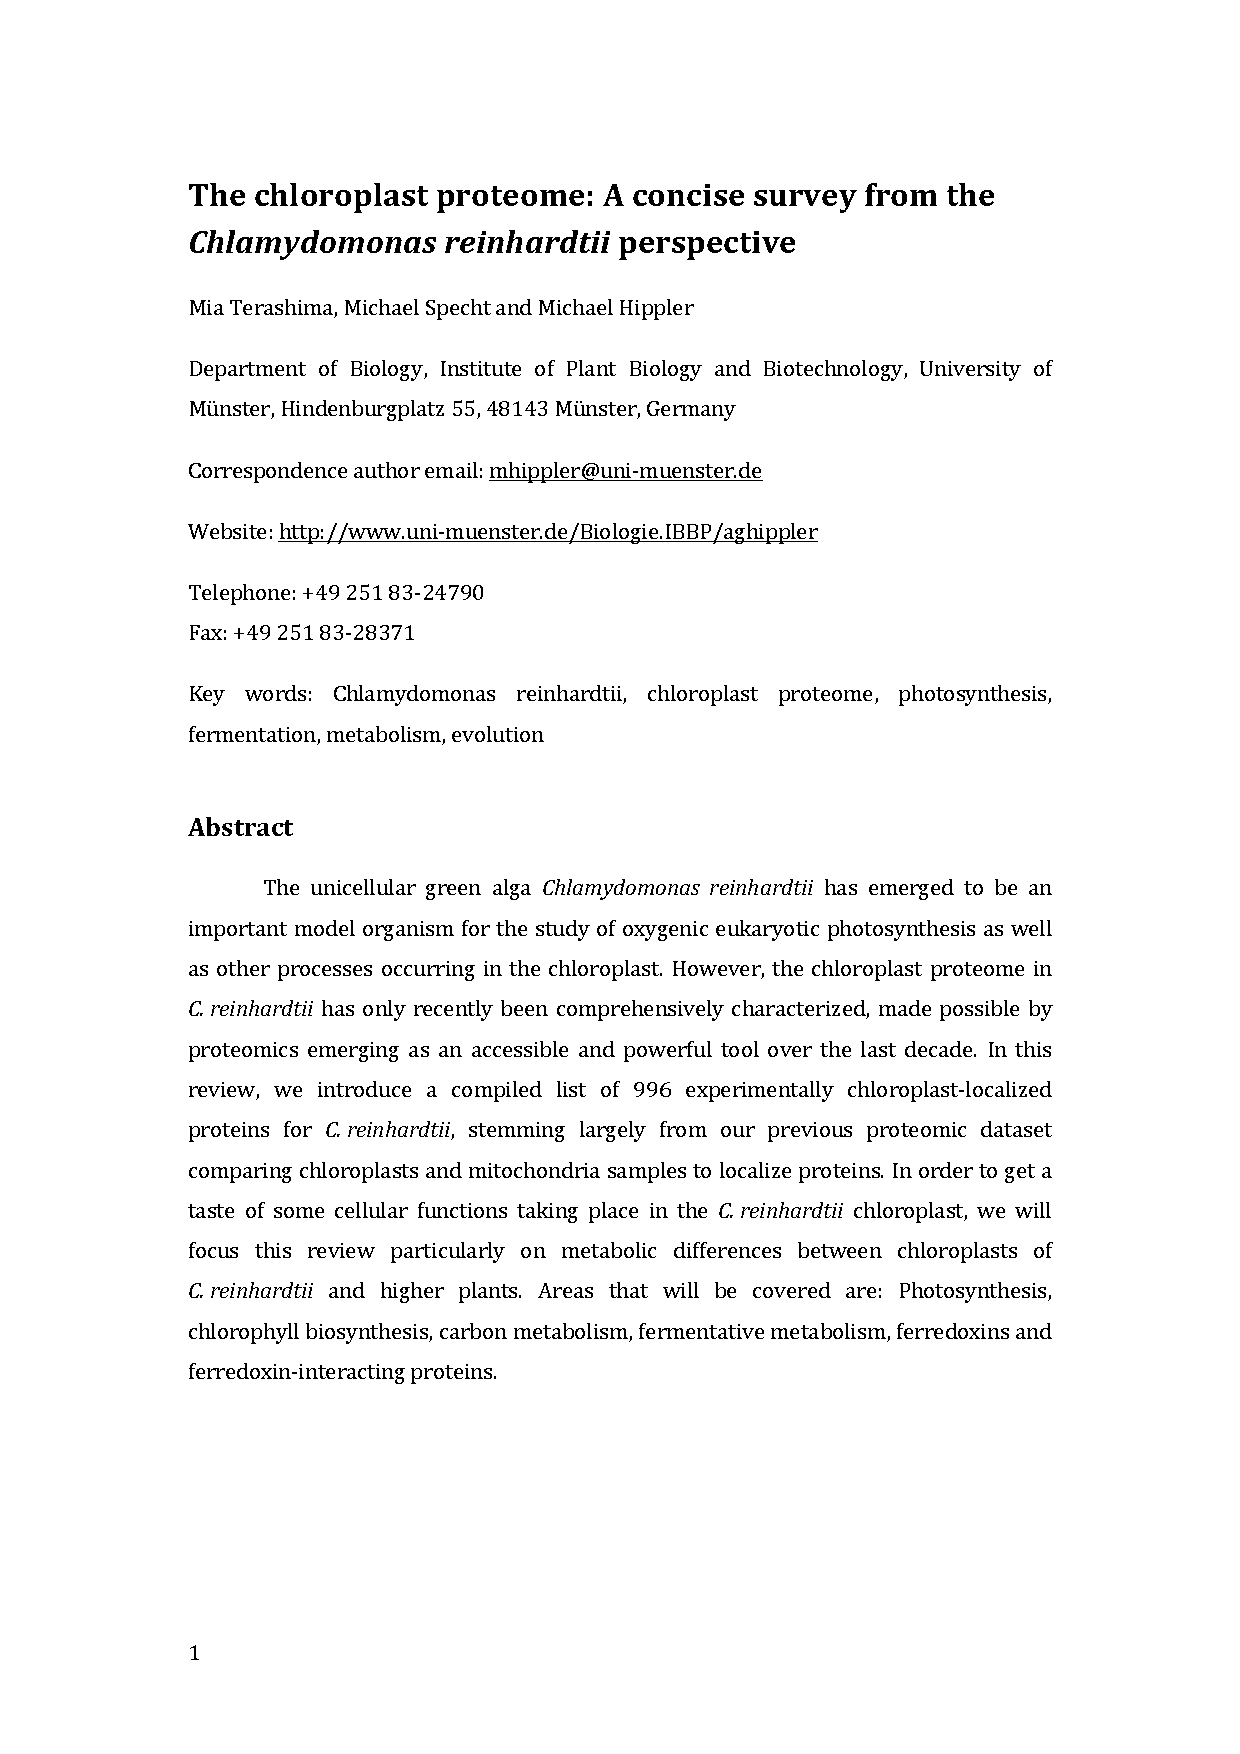
\includepdf{publications/terashima-2011-ms.pdf}

% --------------------------------------------------------------
\cleardoublepage
\section{Concerted action of the new Genomic Peptide Finder and AUGUSTUS allows for automated proteogenomic annotation of the {\em Chlamydomonas reinhardtii} genome}
% \markboth{Concerted action of the new Genomic Peptide Finder and AUGUSTUS allows for automated proteogenomic annotation of the {\em Chlamydomonas reinhardtii} genome}{Concerted action of the new Genomic Peptide Finder and AUGUSTUS allows for automated proteogenomic annotation of the {\em Chlamydomonas reinhardtii} genome}
% \addcontentsline{toc}{section}{Concerted action of the new Genomic Peptide Finder and AUGUSTUS allows for automated proteogenomic annotation of the {\em Chlamydomonas reinhardtii} genome}
% --------------------------------------------------------------

\subsection*{Contributions}

\begin{itemize}
\item what was it, then?
\end{itemize}

% \cleardoublepage
% 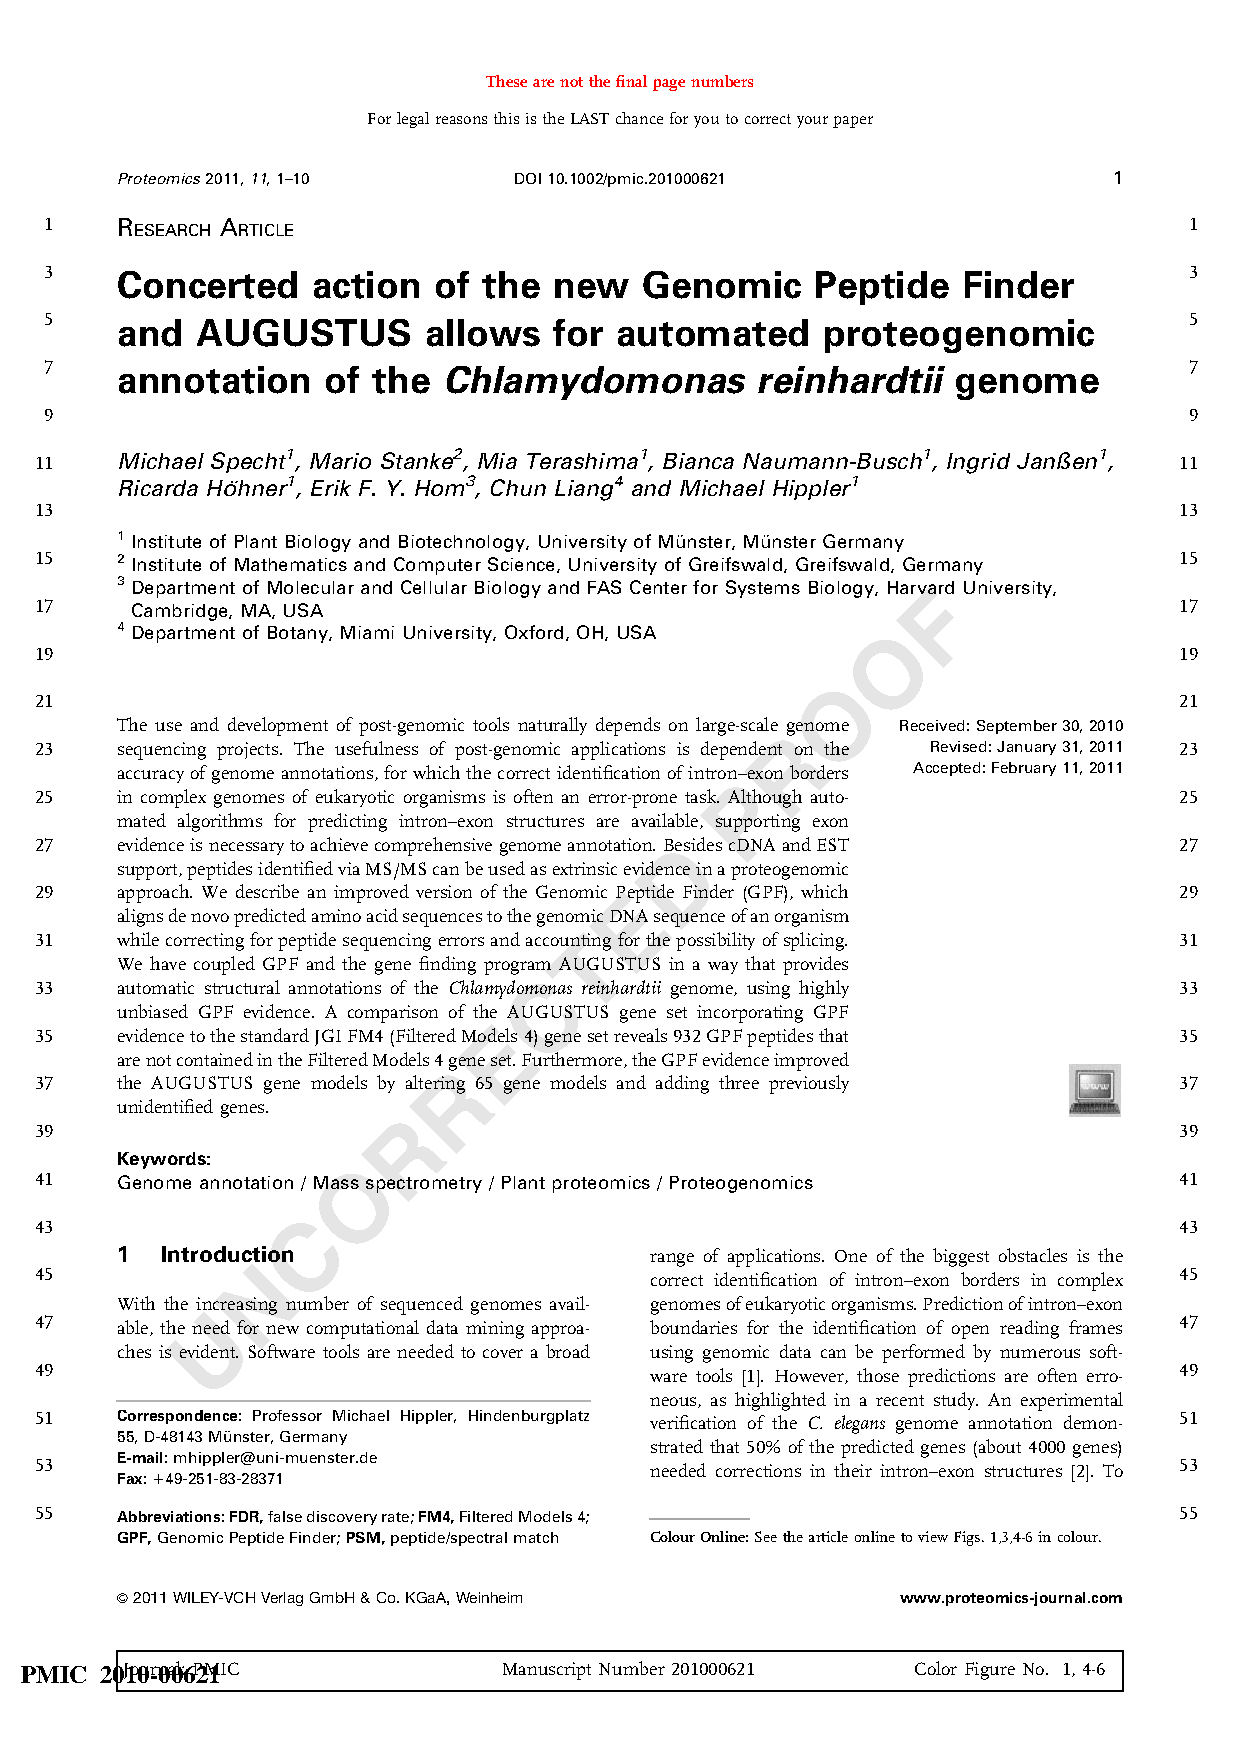
\includepdf{publications/gpf-2011.pdf}

% --------------------------------------------------------------
\cleardoublepage
\section{T.~oceanica paper with Markus Lommer}
% \markboth{T.~oceanica paper with Markus Lommer}{T.~oceanica paper with Markus Lommer}
% \addcontentsline{toc}{section}{T.~oceanica paper with Markus Lommer}
% --------------------------------------------------------------

\subsection*{Contributions}

\begin{itemize}
\item what was it, then?
\end{itemize}

% \cleardoublepage
% \includepdf{publications/lommer-2011.pdf}

% --------------------------------------------------------------
\cleardoublepage
\section{p3d -- Python module for structural bioinformatics}
% \markboth{p3d -- Python module for structural bioinformatics}{p3d -- Python module for structural bioinformatics}
% \addcontentsline{toc}{section}{p3d -- Python module for structural bioinformatics}
% --------------------------------------------------------------

\subsection*{Contributions}

\begin{itemize}
\item what was it, then?
\end{itemize}

% \cleardoublepage
% 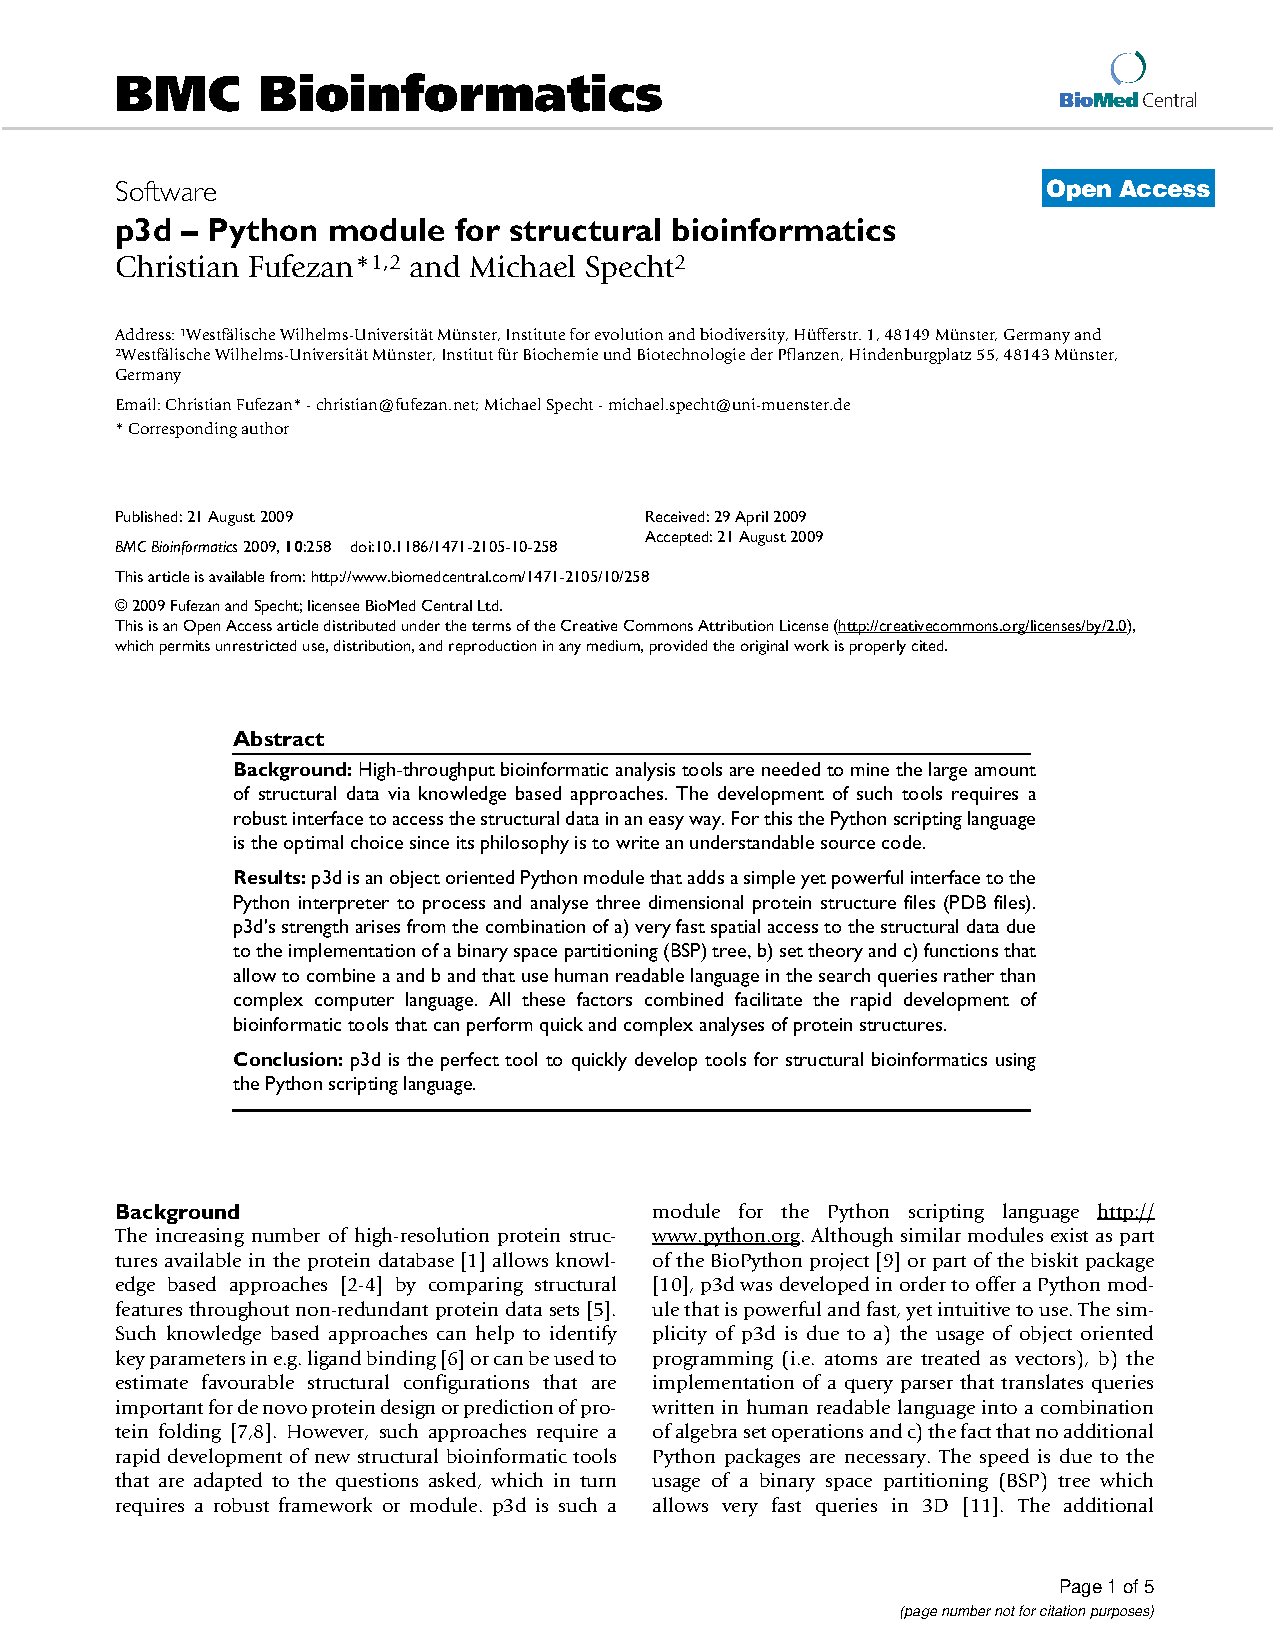
\includepdf{publications/fufezan-2009.pdf}

% ==============================================================
\chapter{Discussion and outlook}
% ==============================================================

Cite \cite{Specht2011}.

% ==============================================================
\chapter{Summary}
% ==============================================================

% ==============================================================
\chapter*{Appendix A: qTrace - Rapid quantitation of metabolically labeled sister peptides}
\markboth{Appendix A: qTrace - Rapid quantitation of metabolically labeled sister peptides}{Appendix A: qTrace - Rapid quantitation of metabolically labeled sister peptides}
\addcontentsline{toc}{chapter}{Appendix A: qTrace - Rapid quantitation of metabolically labeled sister peptides}
% ==============================================================

\begin{figure}[h]
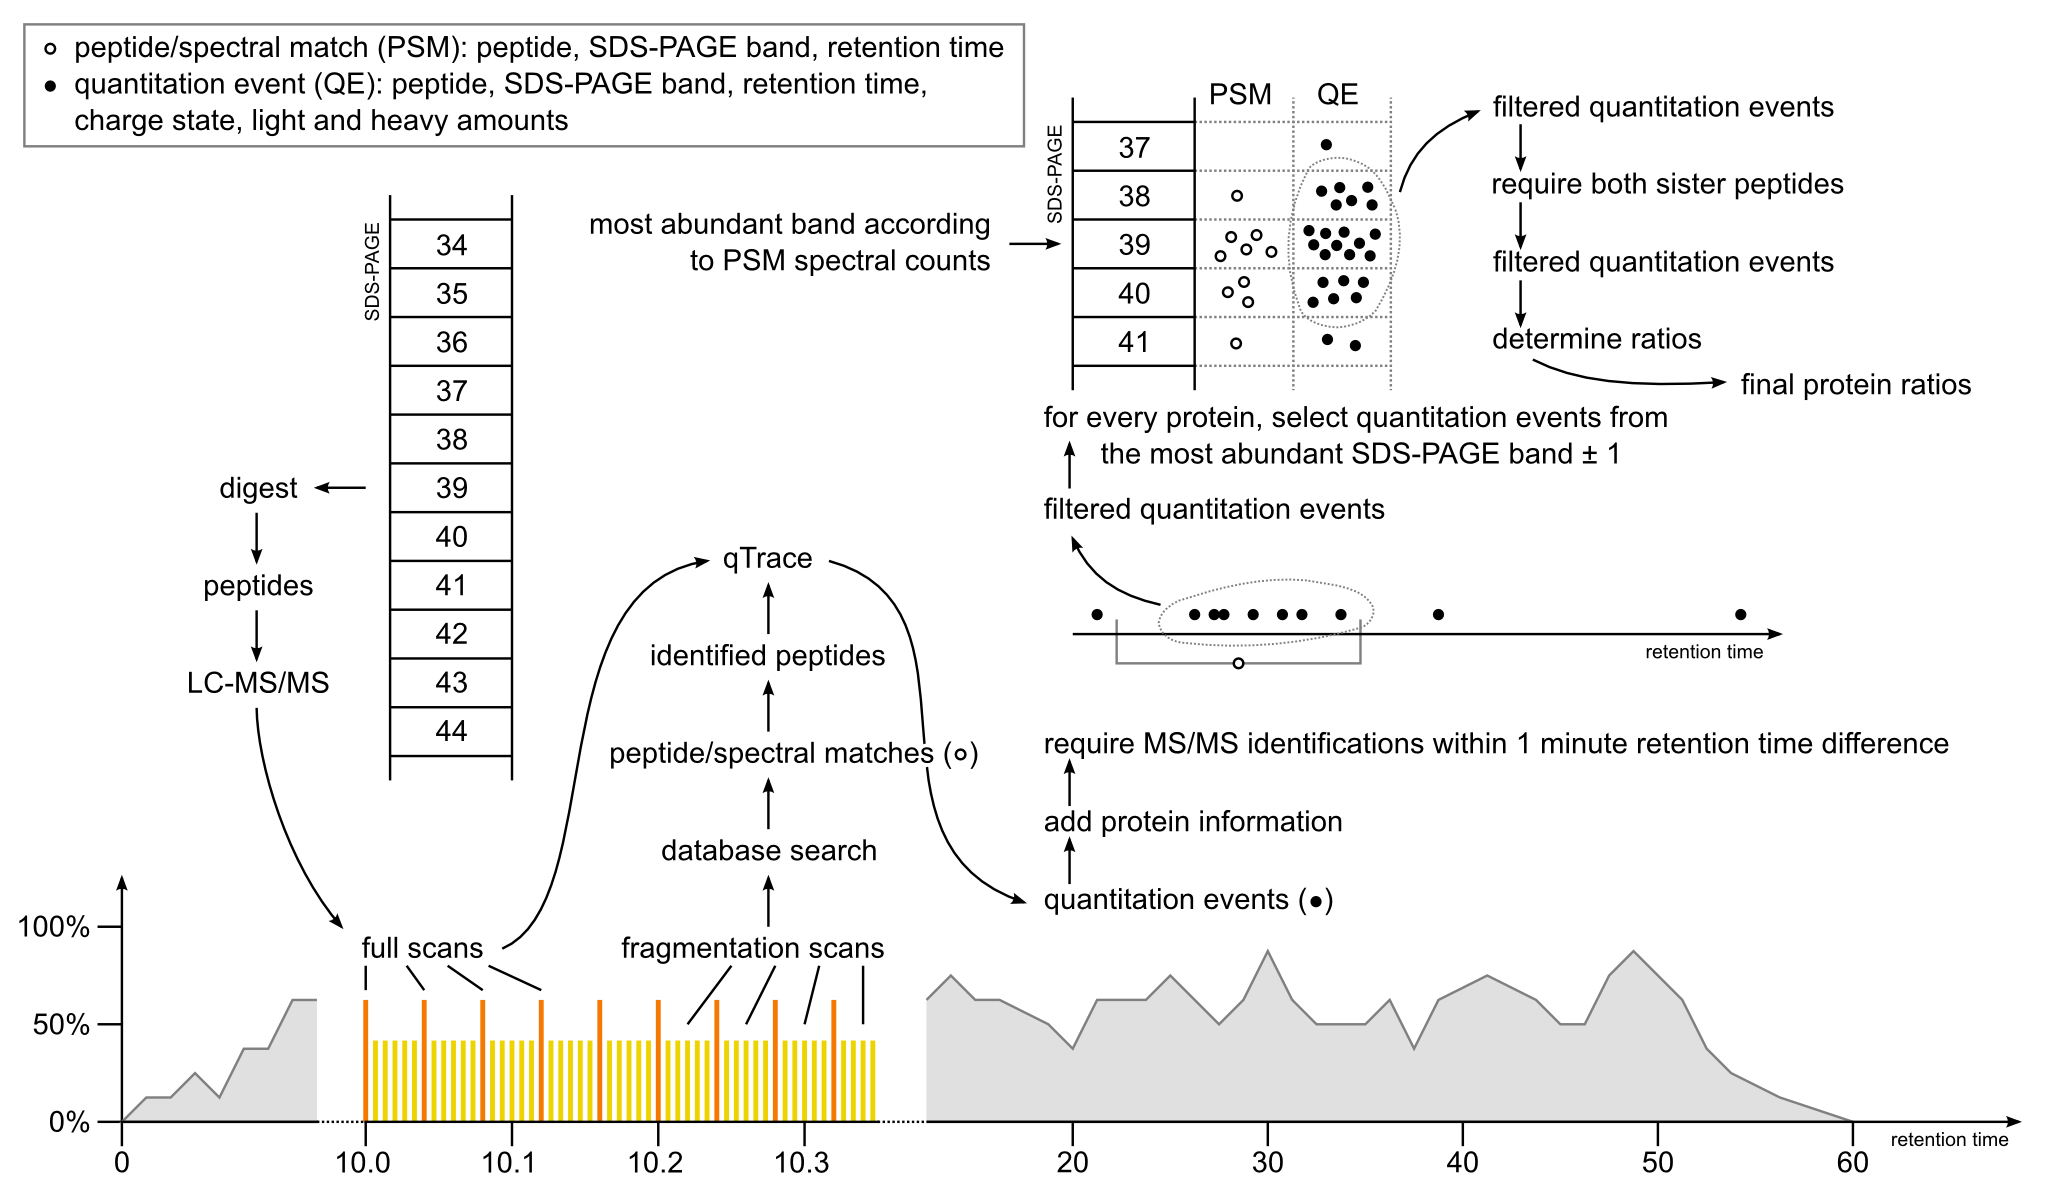
\includegraphics[width=\textwidth]{figures/exp-setup.jpg}
\caption{
{\bf Caption.} 
Caption here.
}
\label{fig:qtrace-workflow}
\end{figure}

% ==============================================================
\chapter*{Appendix B: Proteomatic workflow for proteogenomic genome annotation}
\markboth{Appendix B: Proteomatic workflow for proteogenomic genome annotation}{Appendix B: Proteomatic workflow for proteogenomic genome annotation}
\addcontentsline{toc}{chapter}{Appendix B: Proteomatic workflow for proteogenomic genome annotation}
% ==============================================================

% ==============================================================
\renewcommand{\baselinestretch}{1.0} 
\renewcommand{\arraystretch}{1.0} 
% ==============================================================
\newpage
\bibliography{library}
\addcontentsline{toc}{chapter}{References}
\markboth{References}{References}
\bibliographystyle{unsrt}
    
% ==============================================================
\chapter*{Acknowledgements}
\markboth{Acknowledgements}{Acknowledgements}
\addcontentsline{toc}{chapter}{Acknowledgements}
% ==============================================================

% ==============================================================
\chapter*{Curriculum vitae}
\markboth{Curriculum vitae}{Curriculum vitae}
\addcontentsline{toc}{chapter}{Curriculum vitae}
% ==============================================================

% Michael Specht \\
% Toppheideweg 34 \\
% 48161 Münster
% 
% Phone: +49 251 4808158 \\
% E-mail: \href{mailto:michael.specht@uni-muenster.de}{michael.specht@uni-muenster.de}
% 

\begin{longtable}{@{}lp{12.5cm}}

\cvsubheader{Personal details}

Date of birth: & December 23, 1981 \\
Place of birth: & Magdeburg, Germany \\
Marital status: & married, two children\\
\\

\cvsubheader{Publications}

03/2011 & {\bf Specht M.}, Stanke M., Terashima M., Naumann-Busch B., Janßen I., Höhner R., Hom E. F. Y., Liang C., Hippler M. (2011). Concerted action of the new Genomic Peptide Finder and AUGUSTUS allows for automated proteogenomic annotation of the Chlamydomonas reinhardtii genome. Proteomics, in press. \\

02/2011 & {\bf Specht M.}, Kuhlgert S., Fufezan C., Hippler M. (2011). Proteomics to go: Proteomatic enables the user-friendly creation of versatile MS/MS data evaluation workflows. Bioinformatics 2011; doi: 10.1093/bioinformatics/btr081 (in press). \\

07/2010 & Terashima M., {\bf Specht M.}, Naumann B., Hippler M. (2010). Characterizing the anaerobic response of Chlamydomonas reinhardtii by quantitative proteomics. Mol Cell Proteomics, 9(7), 1514-32. \\

08/2009 & Fufezan C., {\bf Specht M.} (2009). p3d – Python module for structural bioinformatics. BMC Bioinformatics, 10:258. \\

11/2007 & Ropinski T., {\bf Specht M.}, Meyer-Spradow J., Hinrichs K., Preim B. (2007). Surface Glyphs for Visualizing Multimodal Volume Data. Vision, Modelling and Visualization (VMV) (3-13), Saarbrücken, 2007. \\

\cvsubheader{Talks}

\cvtitle{03/2011}{DGMS 2011, Dortmund}
& Proteomics to go: Proteomatic enables the user-friendly creation of versatile MS/MS data evaluation workflows. \\
\tabspace\\

\newpage 

\cvsubheader{Professional experience}

\cvtitle{since 04/2007}{Institute of Plant Biology and Biotechnology\newline Westfälische Wilhelms-Universität Münster}
& Doctoral student in the lab of Prof. Dr. Michael Hippler \newline
% \vspace{6pt}
\vspace{-9pt}
\begin{compactitem}
\item Proteomatic: design and implementation of a user-friendly, decentralized MS/MS data 
evaluation platform \vspace{4pt}\newline
Link: \href{http://www.proteomatic.org}{http://www.proteomatic.org}
% \vspace{-12pt}
% \begin{compactitem}
\item Genomic Peptide Finder: Software for the alignment of MS/MS {\em de novo}
predicted amino acid sequences to the genomic DNA sequence of an organism.
Resulting peptides may be used for evidence-based proteogenomic genome annotation. \vspace{4pt}\newline
Link: \href{http://github.com/specht/gpf}{http://github.com/specht/gpf}.
\item qTrace: Software for the high-throughput quantitation of metabolically
labeled samples (e.g. $^{\textrm{13}}$C Arg SILAC or $^{\textrm{15}}$N) in survey scans.\vspace{4pt}\newline
Link: \href{http://github.com/specht/qtrace}{http://github.com/specht/qtrace}
% \end{compactitem}
\item establishment of free MS/MS data evaluation software in the lab, resulting 
in increased throughput, lower costs and proliferation of MS/MS data 
evaluation-related expertise
\end{compactitem}
% \vspace{-6pt}
\tabspace\\

\cvtitle{10/2006 -- 03/2007}{PROVISIO Software GmbH Münster}
& Software developer -- Realtime Rendering Group \newline
\vspace{-9pt}
\begin{compactitem}
\item design and implementation of a fast JPEG decoder
\item implementation of various user interface widgets for Pictomio
(photo viewer software)
\end{compactitem}
\vspace{-6pt}
\tabspace\\

\cvtitle{07/2005 -- 02/2006}{1komma6 Multimediale Dienstleistungen GmbH Münster}
& Internship -- Web development, focus on accessibility \newline
\tabspace\\

\cvsubheader{Education}
\cvtitle{03/2006 -- 11/2006}{Diploma thesis}
& \emph{Glyph-enhanced Volume Visualization}. \newline
Development of a visualization method for the interactive, simultaneous display 
of multiple, related medical data sets (CT and PET).\tabspace\\
% % \input{../../common-en/chromacoding}
% % \input{../../common-en/studienarbeit}
% 

\cvtitle{10/2001 -- 11/2006}{Study of Computational Visualistics}
& Study of Computational Visualistics (computer science with a focus on computer 
graphics) at the Otto-von-Guericke-Universität Magdeburg.\tabspace\\

\cvtitle{09/2000 -- 07/2001}{Alternative civilian service}
& Civilian service at the retirement home "`Luisenhaus"', Potsdam. \tabspace\\

\cvtitle{09/1992 -- 05/2000}{Secondary school}
& Werner-von-Siemens-Gymnasium, Magdeburg. \tabspace\\

% 
% \newpage
% 
\cvsubheader{Further education}
% 
\cvtitle{10/2010}{Advanced Scientific Programming in Python}
& Participated in an autumn school, held in Trento, Italy,
organized by G-Node, the center for Mind/Brian Sciences, and Fondazione Bruno Kessler.\tabspace\\

\cvsubheader{Miscellaneous projects}
% 
% % \input{../../common-en/nprflow}
% % \input{../../common-en/hamster}
% % \input{../../common-en/tutorium}
% % \input{../../common-en/vib}

\cvtitle{02/2003}{Student anti war group}
& Foundation of the student anti war group at the University of Magdeburg,
shortly before the beginning of the Iraq war in March 2003.
Planning and organization of discussion rounds and movie nights. \tabspace\\

\cvtitle{11/2002 -- 11/2003}{Short film "`pixelle ma belle \#01"'}
& \begin{compactitem}
\vspace{-9pt} 
\item design and implementation of a distributed video rendering software
\item development of an alternative, low-cost blue screen method
\end{compactitem}
\vspace{6pt} 
Link: \href{http://www.pixellemabelle.de}{www.pixellemabelle.de}
\tabspace\\

% % \input{../../common-en/fx}
% % \input{../../common-en/ferienlager}
% % \input{../../common-en/zeitnahme}
% 
\cvsubheader{Skills}
% 

foreign languages
& English (fluent)\newline
French (basic knowlegde) \tabspace\\

programming
& C, C+\kern-0.2em +, Qt, Ruby, Python, PHP, Java, Assembler, XHTML, CSS, Ajax, MySQL\tabspace\\

software
& Linux, Windows, Mac OS X \newline
Visual Studio, Microsoft Office, OpenOffice, \LaTeX, Photoshop, GIMP, Inkscape \newline
CVS, Subversion, Git\tabspace\\

% 
\end{longtable}
% 

\end{document}
